\section{Background and Preliminary}
\label{sec:background}
UPRESSO is compatible with OIDC, and achieves the privacy protection based on the discrete logarithm problem.
Here, we provide a brief introduction on OIDC and the discrete logarithm problem.

\subsection{OpenID Connect}
\label{subsec:OIDC}
%To be compatible with existing SSO systems, UPRESSO is designed on top of OpenID Connect (OIDC)~\cite{OpenIDConnect}, one 
OIDC~\cite{OpenIDConnect} is an extension of OAuth 2.0 to support user authentication,
 and becomes one of the most prominent SSO authentication protocols.
%original by chengqian guo
%To be compatible with existing SSO systems, UPRESSO is designed on top of OpenID Connect (OIDC)~\cite{OpenIDConnect}, one of the most prominent SSO authentication protocols~\cite{SAMLIdentifier}. Here, we use the implicit flow of OIDC as an example to describe the authentication flows in SSO. Moreover, our proposed framework can also work for other flows with only minor modifications.
%As a typical SSO authentication protocol,
Same as other SSO protocols~\cite{SAMLIdentifier}, OIDC involves three entities, i.e., {\em users}, {\em identity provider (IdP)}, and {\em relying parties (RPs)}.
Both users and RPs have to register at the IdP,    
the users register at the IdP to create credentials and identifiers (e.g. $ID_U$), %which are securely maintained by the IdP.
while each RP registers at the IdP with its endpoint information to create its unique identifier (e.g., $ID_{RP}$) and the corresponding credential.
IdP is assumed to securely maintain the attributes  of users and RPs.   
Then, in the SSO authentication sessions, 
 each user is responsible to start a login request at an RP, redirect the messages between RP and IdP, and check the scope of user's attributes provided to the RP;
 IdP authenticates the user (if the user has not been authenticated), sets the $PPID$ for the user $ID_U$ at the RP $ID_{RP}$,
 constructs the identity proof with  $PPID$, $ID_{RP}$ and the user's attributes consented by the user, and finally transmits the identity proof to the RP's registered endpoint (e.g., URL);
 each RP constructs an identity proof request with its identifier and the requested scope of  user's attributes, sends an identity proof request to the IdP through the user, and parses the received identity proof to authenticate and authorize the user.
Usually, the redirection and checking at the user are handled by a user-controlled software, called {\em user agent} (e.g., browser).



%original by chengqian guo
%OIDC is an extension of OAuth 2.0 to support user authentication. As a typical SSO authentication protocol, OIDC involves three entities, i.e., {\em users}, {\em identity provider (IdP)}, and {\em relying parties (RPs)}. Users register at the IdP to create credentials and identifiers (e.g. $ID_U$), which are securely maintained by the IdP. Moreover, an RP also has to register at the IdP with its endpoint information to create its unique identifier. During an SSO process, a user is also responsible for redirecting the identity proof request from the RP to the IdP, checking the scope of user attributes in the identity proof returned by the IdP, and forwarding it to the RP. Usually, the redirection and checking are handled by a user-controlled software, called {\em user agent} (e.g., browser). The IdP maintains user credentials and attributes. Once requested, it authenticates the user and generates the identity proof, which contains user identifier (e.g., $PPID$ in OIDC), RP identifier (e.g. $ID_{RP}$), and a set of user attributes that the user consents to share with the RP. The identity proof is then returned to the registered endpoint of the RP (e.g., URL). RP can be any web server that provides continuous and personalized services to its users. When a user attempts to log in, the RP sends an identity proof request to the IdP through the user, and parses the received identity proof to authenticate and authorize the user.


%****** Add discussion about why implicit flow is used in this work
\noindent\textbf{Implicit flow of user login.}
OIDC supports three processes for the SSO authentication session, known as {\em implicit flow}, {\em authorization code flow} and {\em hybrid flow} (i.e., a mix-up of the previous two).
In the implicit flow of OIDC, a token, known as {\em id token}, is introduced as the identity proof, which contains user identifier (i.e., $PPID$), RP identifier (i.e., $ID_{RP}$), the issuer (i.e., IdP), issuing time, the validity period, and other requested attributes. The IdP signs the id token using its private key to ensure integrity, and sends it through the user to RP.
In the authorization code flow, IdP binds an authorization code with the RP, and redirects this code to the RP;
 then RP establishes an HTTPS connection with IdP to ensure the integrity and confidentiality of the identity proof, and  uses the authorization code with the RP's credential to obtain PPID and the user's other  attributes.

UPRESSO is compatible to all the three flows.
For brevity, we will present the application of UPRESSO in the implicit flow in details, and provide the integration with the authorization code flow briefly. 
Here, we first introduce the original processes in the implicit flow of OIDC.
%Moreover, our proposed framework can also work for other flows with only minor modifications.
\begin{figure}[t]
  \centering
  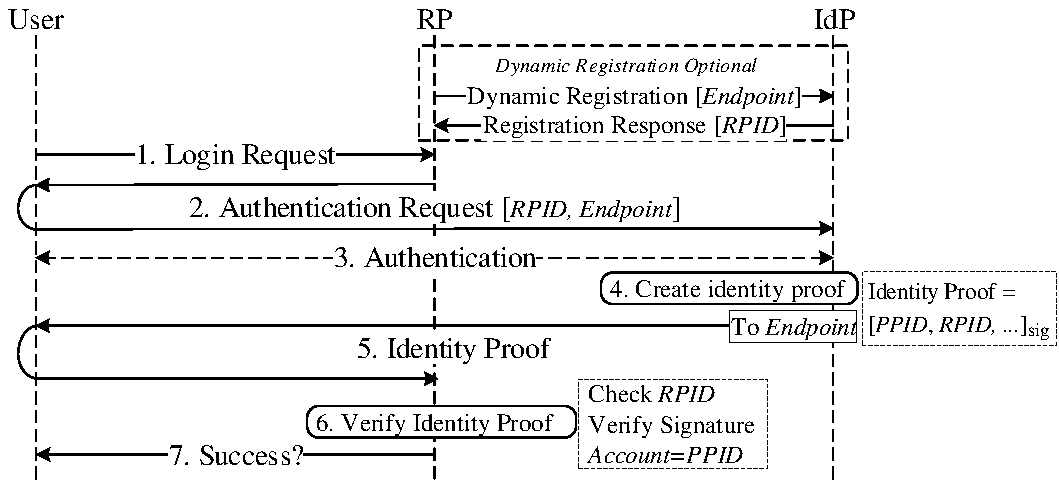
\includegraphics[width=\linewidth]{fig/OIDC1.pdf}
  %\subfigure[Authorization Code Flow]{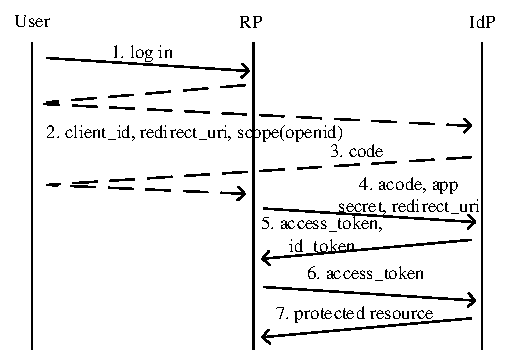
\includegraphics[width=\linewidth]{fig/openidconnect2.pdf}\label{fig:OpenID_code}}
  %\subfigure[Hybrid Flow]{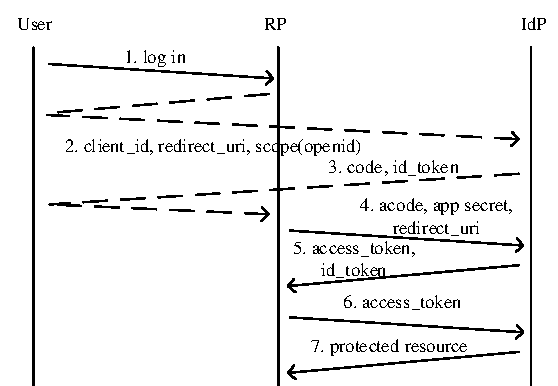
\includegraphics[width=\linewidth]{fig/openidconnect3.pdf}\label{fig:OpenID_hybrid}}
  \caption{The implicit protocol flow of OIDC.}
  \label{fig:OpenID}
\end{figure}
As shown in Figure~\ref{fig:OpenID}, the implicit flow of OIDC consists of 7 steps: when a user attempts to log in to an RP (Step 1), the RP constructs a request for identity proof, which is redirected by the user to the corresponding IdP (Step 2). The request contains $ID_{RP}$, RP's endpoint and a set of requested user attributes. If the user has not been authenticated yet, the IdP performs an authentication process (Step 3). If the RP's endpoint in the request matches the one registered at the IdP, it generates an identity proof (Step 4) and sends it back to the RP (Step 5). Otherwise, IdP generates a warning to notify the user about potential identity proof leakage. The RP verifies the id token (Step 6), extracts user identifier from the id token and returns the authentication result to the user (Step 7).



\begin{figure}[t]
  \centering
  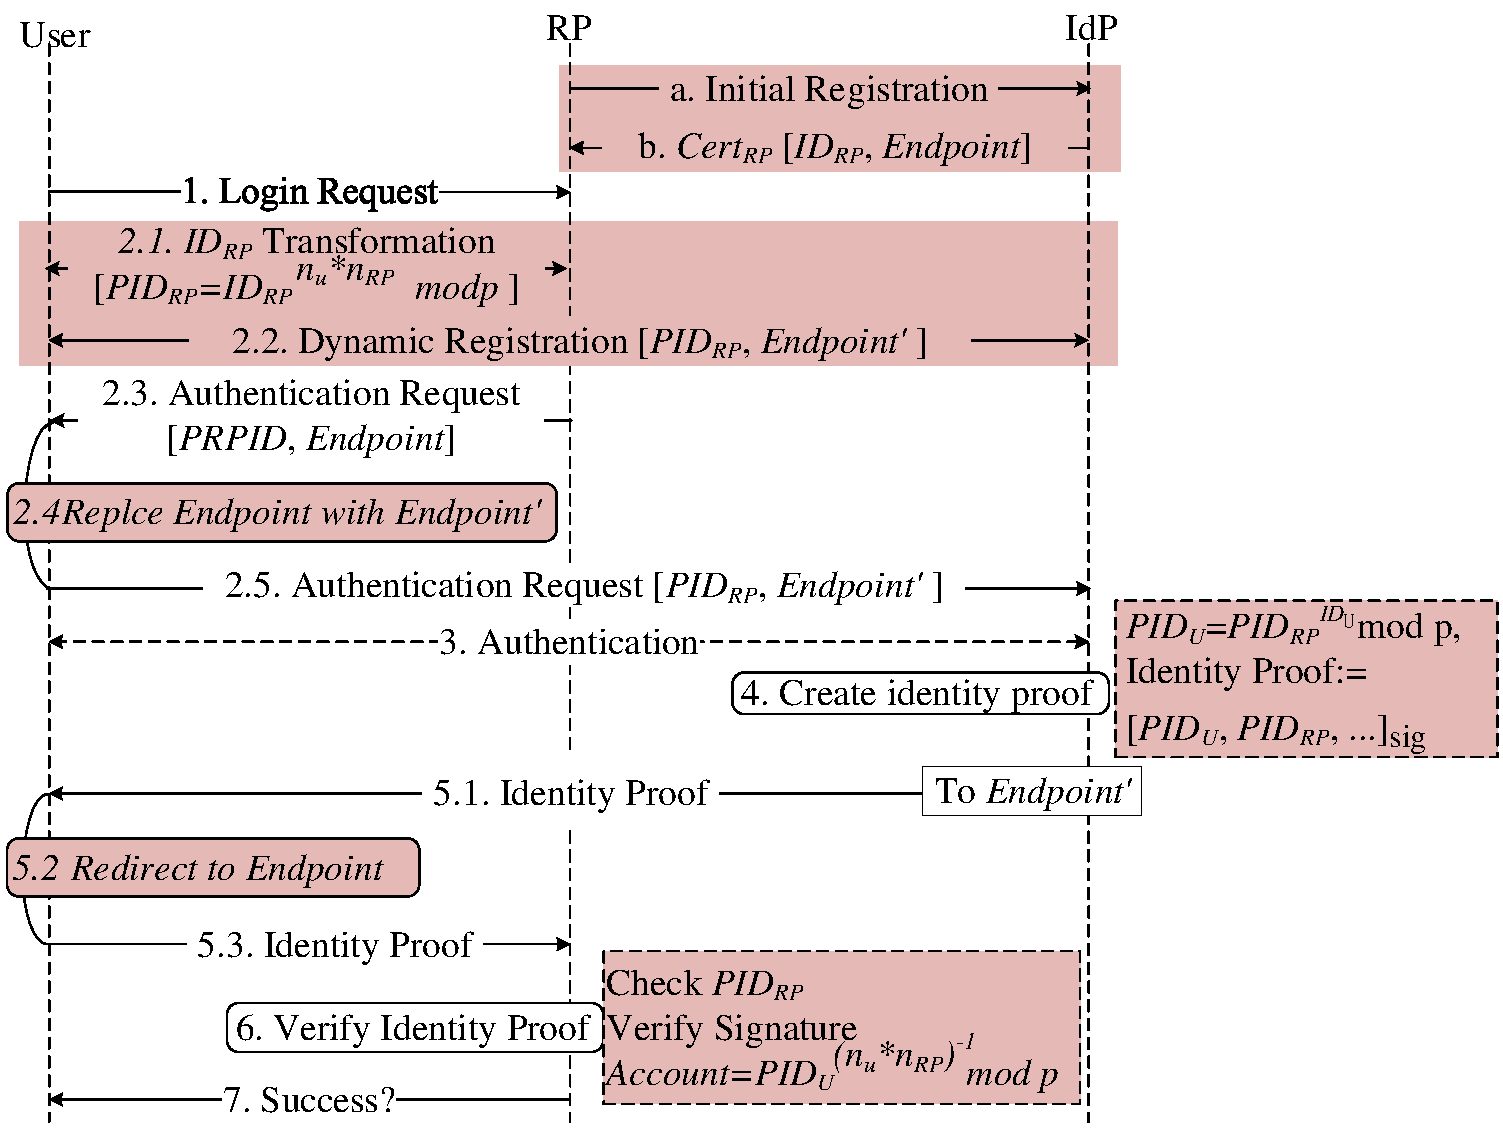
\includegraphics[width=\linewidth]{fig/overview1.pdf}
  %\subfigure[Authorization Code Flow]{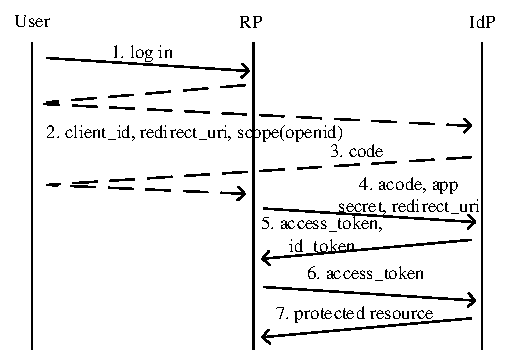
\includegraphics[width=\linewidth]{fig/openidconnect2.pdf}\label{fig:OpenID_code}}
  %\subfigure[Hybrid Flow]{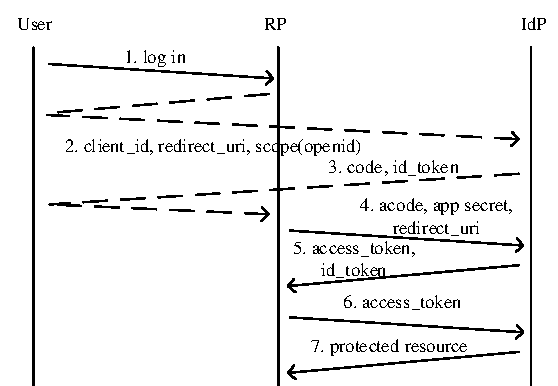
\includegraphics[width=\linewidth]{fig/openidconnect3.pdf}\label{fig:OpenID_hybrid}}
  \caption{The UPRESSO.}
  \label{fig:UPRESSO}
\end{figure}

\noindent\textbf{RP dynamic registration.} OIDC provides a dynamic registration mechanism~\cite{DynamicRegistration} for the RP to renew its $ID_{RP}$ dynamically. % shown in Figure~\ref{fig:OpenID}.
When an RP first registers at the IdP, it obtains a registration token, with which the  RP can invoke the dynamic registration process to
%After a successful initial registration, RP obtains a registration token from the IdP, and
update its information (e.g., the endpoint). % by a dynamic registration process with the  registration token. %which enables the RP to integrate the service provided by IdP,
After each successful dynamic registration, the RP obtains a new unique $ID_{RP}$ from the IdP.
In UPRESSO, we slightly modify dynamic registration to register $PID_{RP}$ at IdP. 
%support the dynamic generated privacy-preserving RP identifier (e.g. $PID_{RP}$).


\subsection{Discrete Logarithm Problem}
\label{sec:dlp}
Discrete logarithm problem is adopted in UPRESSO for the construction of $F_{PID_{RP}}$ and $F_{PID_U}$,
 which generate privacy-preserving user identifier (e.g. $PID_U$) and RP identifier (e.g. $PID_{RP}$) respectively.
Here, we provide a brief description of the discrete logarithm problem.

A number $g$ ($0<g<p$) is called a primitive root modular a prime $p$, if for ${\forall}y$ ($0<y<p$), there is a  number $x$ ($0\le x <p-1$) satisfying $y=g^x \pmod p$.
And, $x$ is called the discrete logarithm of $y$ modulo $p$. Given a large prime $p$, a primitive root $g$ and a number $y$, it is computationally infeasible to derive the discrete logarithm (here $x$) of $y$ (detailed in~\cite{WXWM}), which is called discrete logarithm problem.
The hardness of solving discrete logarithm has been a base of the security of several security primitives, including Diffie-Hellman key exchange and Digital Signature Algorithm (DSA).

In the process of $F_{PID_{RP}}$ and $F_{PID_U}$, we needs to calculate the primitive root for a  large prime $p$ as follows~\cite{Shoup,Wang}.
First, we retrieve a primitive root $g_m$  modulo $p$ by performing the primitive root checking on all the integers one by one. 
 A lemma is propose to simply the checking, that if $p=2q+1$ ($q$ is a prime),  an integer $\mu \in (1, p-1)$ is a primitive root if and only if $\mu^2\neq 1 \ mod \ p$ and $\mu^q\neq 1 \ mod \ p$.
Then, based on $g_m$, we can calculate a new primitive root $g = g_{m}^{t} mod \ p$, where $t$ is an integer coprime to $p-1$.
 
%The details are provided in~\cite{Shoup,Wang}.

%Given a large prime $p$, its primitive root $g$ and a number $y$, it is computationally infeasible to derive the discrete logarithm $x$ of $y$ that satisfies  $g^x = y mod p$ (detailed in~\cite{WXWM}), which is called discrete logarithm problem. The hardness of solving discrete logarithm has been a base of the security of several security primitives, including Diffie-Hellman key exchange and Digital Signature Algorithm (DSA). The $PID_U$ and $PID_{RP}$ generation is based on the modular exponentiation, which requires the parameters, such as $ID_{RP}$ and $PID_{RP}$, to be the primitive root mod $p$ to prevent the user and RP' identity leakage. To calculate the primitive root for a given large prime $p$, we retrieve a primitive root $g_m$ mod $p$, and then calculate the $g = g_{m}^{t} mod \ P$, so that $g$ is another primitive root mod $p$ where $t$ is an integer coprime to $p-1$.


\begin{comment}
%, to prevent IdP from inferring $ID_{RP}$ from $PID_{RP}$, and allow the RP to derive $Account$ from $PID_U$ without obtaining the $ID_U$.
Here, we provide a brief description of the discrete logarithm problem.
A number $g$ ($0<g<p$) is called a primitive root modular a prime $p$, if for ${\forall}y$ ($0<y<p$), there is a  number $x$ ($0\le x <p-1$) satisfying $y=g^x \pmod p$.
And, $x$ is called the discrete logarithm of $y$ modulo $p$. Given a large prime $p$ and a number $y$, it is computationally infeasible to derive the discrete logarithm (here $x$) of $y$ (detailed in~\cite{WXWM}), which is called discrete logarithm problem. The hardness of solving discrete logarithm has been a base of the security of several security primitives, including Diffie-Hellman key exchange and Digital Signature Algorithm (DSA).
To calculate the primitive root for a given large prime $p$,  we retrieve the least primitive root $g_m$  mod $p$,
and then calculate the primitive root $g = g_{m}^{t} mod \ P$, where $t$ is an integer coprime to $p-1$.
A lemma is proposed to check whether an integrity $\mu$ is the primitive root modulo $p$ where $p=2q+1$ ($q$ is a prime), that is,  an integer $\mu \in (1, p-1)$ is a primitive root if and only if $\mu^2\neq 1 \ mod \ p$ and $\mu^q\neq 1 \ mod \ p$~\cite{Shoup,Wang}.
%The details are provided in~\cite{Shoup,Wang}.
\end{comment}

